\chapter{A Matriz de uma Transformação  Linear}
\thispagestyle{empty}

\section{Introdução}
O objetivo deste tópico é  possibilitar o trabalho com  transformações lineares através do estudo de  matrizes associadas a essas transformações. A abordagem do estudo de tranformações lineares via matrizes é interessante por que, de um modo geral, os problemas fundamentais da álgebra linear, a resolução de sistemas lineares e cálculo de autovalores e autovetores, se reduzem ao  trabalho com matrizes.


Inicialmente note que dada uma matriz $A$ de ordem $m\times n$ podemos definir uma aplicação $T_A: \mathbb{R}^n \rightarrow \mathbb{R}^m$ por
\begin{align}
T_A(x)=Ax \label{matrizTa}
\end{align}
para todo $x=(x_1, x_2, ..., x_n) \in \mathbb{R}^n$. Para tornar compatível as operações matriciaiso o vetor $x$ é tomado como a matriz coluna $x=\left[ \begin{array}{c}x_1 \\ x_2 \\ \vdots \\ x_n\end{array} \right]$.

%\textbf{Proposição.}
 A aplicação $T_A$ definida em \eqref{matrizTa} é uma transformação  linear.  De fato, sejam  $x$ e $y$  vetores pertencentes ao $\mathbb{R}^n$ e  $\alpha$ um escalar. Usando a definição de $T_A$ e as  propriedades das operações matriciais,  temos $$T_A(x+\alpha y)=A(x+\alpha y)=Ax+\alpha Ay=T_A(x)+\alpha T_A(y).$$
Ou seja, $T_A$ é linear.  Dessa forma, a cada matriz $A$ de ordem $m\times n$ podemos associar uma transformação linear  $T_A: \mathbb{R}^n \rightarrow \mathbb{R}^m$. A recíproca dessa afirmação também é verdadeira. Isto é, a cada transformação linear $T: \mathbb{R}^n \rightarrow \mathbb{R}^m$ podemos associar uma matriz $A$ de ordem $m\times n$.


A seguir veremos  que esse resultado pode ser  generalizado  para transformações  lineares quaisquer, entre espaços vetoriais de dimensão finita quaisquer. Também veremos  um  procedimento para obter  a matriz de uma transformação linear qualquer.

\section{A Matriz de uma Transformação Linear}


Sejam $U$ e $V$ espaços vetoriais sobre $\mathbb{R}$,  $T: U \rightarrow V$ uma transformação linear, $\alpha=\{ u_1, u_2, ...,u_n\}$ uma base $U$ e $\beta=\{v_1, v_2, ...,v_m\}$ uma base de $V$.  Dessa forma, dado $u\in U$, existem  únicos escalares $a_1$, $a_2$,...,$a_n$ tais que

\begin{align}
u&=a_1u_1+ a_2u_2+ ...+a_nu_n .
\end{align}

Como $T$ é linear, então obtemos

\begin{align}
T(u)&=a_1T(u_1)+ a_2T(u_2)+ ...+a_nT(u_n).
\end{align}

%Além disso, como $T(u) \in V$ existem  únicos escalares $b_1$, $b_2$,...,$b_n$ tais que
%
%\begin{align}
%T(u)&=b_1v_1+ b_2v_2+ ...+b_mv_m .
%\end{align}

Mais adiante voltaremos as equações (1) e (2). Por enquanto, observe que como $T(u_1)$,  $T(u_2)$,...,$T(u_n)$ são vetores de $V$,  então existem escalares $a_{ij}$, com $1\leq i \leq m$  e $1\leq j \leq n$ tais que

\begin{align}
T(u_1)&=a_{11}v_1+ a_{21}v_2+ ...+a_{m1}v_m \nonumber \\
T(u_2)&=a_{12}v_1+ a_{22}v_2+ ...+a_{m2}v_m \nonumber \\
      \vdots&= \vdots \\
T(u_n)&=a_{1n}v_1+ a_{2n}v_2+ ...+a_{mn}v_m \nonumber
\end{align}

Daí obtemos a matriz de coordenadas (ou vetor de coordenadas, já que possui uma única coluna), em relação a base $\beta$, de $T(u_1)$, $T(u_2)$,..., $T(u_n)$. Isto é,

$[T(u_1)]_{\beta}=\left[ \begin{array}{c}a_{11} \\ a_{21} \\ \vdots \\ a_{m1}\end{array} \right]$, $[T(u_2)]_{\beta}=\left[ \begin{array}{c}a_{12} \\ a_{22} \\ \vdots \\ a_{m2}\end{array} \right]$, ..., $[T(u_n)]_{\beta}=\left[ \begin{array}{c}a_{1n} \\ a_{2n} \\ \vdots \\ a_{mn}\end{array} \right]$.


\vspace{1cm}

\textbf{Definição (Matriz de uma tranformação linear).}  A matriz da transformação linear $T: U \rightarrow V$ em relação às bases $\alpha$ e $\beta$, denotamos $[T]_{\beta}^{\alpha}$, é a matriz cujas colunas são formadas pelos elementos das matrizes de coordenadas $ [T(u_1)]_{\beta},  [T(u_2)]_{\beta},..., [T(u_n)]_{\beta}$. Isto é,
\vspace{0.3cm}
$$[T]_{\beta}^{\alpha}=\left[ \begin{array}{cccc}a_{11} &a_{21} & \hdots & a_{1n} \\ a_{21} & a_{22} & \hdots & a_{2n} \\ \vdots & \vdots & \ddots & \vdots \\ a_{m1}& a_{m_2} & \hdots & a_{mn} \end{array} \right].$$


\subsection{Exemplos}

\begin{enumerate}
\item
Sejam $\alpha=\{ (1,1), (-1,1)\}$ uma base $\mathbb{R}^2$,  $\beta=\{(1,1,1), (1,1,0),(1,0,0)\}$ uma  base de $\mathbb{R}^3$  e $T: \mathbb{R}^2 \rightarrow \mathbb{R}^3$ e  a transformação linear definida por $T(x,y,z)=(x,x+y,y)$. Determine a matriz  de $T$ em relação as bases ${\alpha}$ e ${\beta}$. Isto é, $[T]_{\beta}^{\alpha}$.

\vspace{0.5cm}
\noindent\textit{Resolução.} Por definição,  $[T]_{\beta}^{\alpha}$ é  a matriz cujas colunas são formadas pelos vetores  $[T(1,1)]_{\beta}$  e  $[T(-1,1)]_{\beta}$, nessa ordem. Logo, precisamos calcular primeiro $T(1,1)$ e $T(-1,1)$ e em seguida as suas coordendas em relação a base $\beta$.

\vspace{0.5cm}
\textbf{1. Cálculo de  $T(1,1)$ e de suas coordenadas na base $\beta$, $[T(1,1)]_{\beta}$.}

Como $T(1,1)=(1, 2, 1)$, devemos calcular $a_{1}$, $a_{2}$ e $a_{3}$, tais que,

\begin{align*}
(1,2,1)&=a_1(1, 1, 1)+a_2(1,1,0)+a_3(1,0,0), \\
(1,2,1)&=(a_1+a_2+a_3, a_1+a_2,a_1).
\end{align*}
Daí  obtemos o sistema linear
\begin{align*}
a_1+a_2+a_3 &=1 \\
a_1+a_2 &=2 \\
a_1&= 1,
\end{align*}
cuja solução é $a_1=-1$, $a_2=1$ e $a_3=-1$. De onde obtemos
$[T(1,1)]_{\beta}=\left[ \begin{array}{c}-1 \\ 1 \\ -1\end{array} \right]$.

\vspace{0.5cm}
\textbf{2. Cálculo de  $T(-1,1)$ e de suas coordenadas na base $\beta$, $[T(-1,1)]_{\beta}$.}

Como $T(-1,1)=(-1, 0, 1)$, devemos calcular $a_{1}$, $a_{2}$ e $a_{3}$, tais que,

\begin{align*}
(-1,0,1)&=a_1(1, 1, 1)+a_2(1,1,0)+a_3(1,0,0), \\
(-1,0,1)&=(a_1+a_2+a_3, a_1+a_2,a_1).
\end{align*}

Analogamente, ao primeiro caso, resolvemos  o sistema linear
\begin{align*}
a_1+a_2+a_3 &=-1 \\
a_1+a_2 &=0 \\
a_1&= 1,
\end{align*}
cuja solução é $a_1=0$, $a_2=0$ e $a_3=-1$ e  obtemos
$[T(-1,1)]_{\beta}=\left[ \begin{array}{c}0 \\0\\ -1\end{array} \right]$.

\textbf{3. Escrevemos a matriz de $T$.}

Finalmente, temos a matriz $$[T]_{\beta}^{\alpha}=\left[ \begin{array}{cc}-1 &0 \\ \;\;1 &0  \\  -1& -1 \end{array} \right].$$

%$$[T]_{\beta}^{\alpha}=\left[ \begin{array}{cc}a_{11} &a_{12} \\ a_{21} & a_{22}  \\  a_{31}& a_{32} \end{array} \right].$$

\item Dado  $\alpha =\{e_1, e_2, e_3, e_4\}$ a base canônica do $ \mathbb{R}^4 $ e $\beta=\{(1,1,1), (0,1,1),(0,0,1)\}$ uma base do $ \mathbb{R}^3$, determinar a transformação linear  $T: \mathbb{R}^4 \rightarrow \mathbb{R}^3$  tal que
$$[T]_{\beta}^{\alpha}=\left[ \begin{array}{cccc}1 &2&3&0 \\ -1 &0&1&1  \\  5&4&0&-2 \end{array} \right].$$

\vspace{0.5cm}
\noindent\textit{Resolução.}  Primeiro note que pela definição de  $[T]_{\beta}^{\alpha}$ , temos:

$[T(e_1)]_{\beta}=\left[ \begin{array}{c}1 \\-1\\ 5\end{array} \right]$, $[T(e_2)]_{\beta}=\left[ \begin{array}{c}2 \\0\\ 4\end{array} \right]$,$[T(e_3)]_{\beta}=\left[ \begin{array}{c}3\\1\\ 0\end{array} \right]$ e $[T(e_4)]_{\beta}=\left[ \begin{array}{c}0 \\1\\ -2\end{array} \right]$.
Dessa maneira, obtemos:
\begin{align*}
T(e_1)&=1(1, 1, 1)+(-1)(0,1,1)+5(0,0,1)=(1,0,6), \\
T(e_2)&=2(1, 1, 1)+0(0,1,1)+4(0,0,1)=(2,2,6), \\
T(e_3)&=3(1, 1, 1)+1(0,1,1)+0(0,0,1)=(3,4,4), \\
T(e_4)&=0(1, 1, 1)+1(0,1,1)+(-2)(0,0,1)=(0,1,-1).
\end{align*}

Agora o problema se reduz a encontrar uma transformação linear $T: \mathbb{R}^4 \rightarrow \mathbb{R}^3$ tal que
 \begin{align*}
T(e_1)&=(1,0,6), \\
T(e_2)&=(2,2,6), \\
T(e_3)&=(3,4,4), \\
T(e_4)&=(0,1,-1).
\end{align*}
Para isto, consideremos um vetor genérico do $ \mathbb{R}^4$, isto é, $(x,y,z,w)$ e vamos escrevê-lo como combinação linear dos vetores da base $\alpha =\{e_1, e_2, e_3, e_4\}$. Ou seja, $$(x,y,z,w)= xe_1+ y e_2+z e_3+ we_4.$$
Como $T$ é linear, obtemos:
\begin{align*}
T(x,y,z,w)&= xT(e_1)+ y T(e_2)+z T(e_3)+ wT(e_4),\\
                &= x(1,0,6)+ y (2,2,6)+z (3,4,4)+ w(0,1,-1),\\
               &=(x+2y+3z, 2y+4z+w,6x+6y+4z+w).
\end{align*}

Portanto, a transformação linear procurada é  $$T(x,y,z,w)=(x+2y+3z, 2y+4z+w,6x+6y+4z+w).$$


\item \textbf{Matriz da transformação Identidade e a matriz mudança de base.} Sejam $\alpha =\{u_1, u_2, ..., u_n\}$ e $\beta =\{v_1, v_2, ..., v_n\}$ duas bases distintas de $U$   e  $T:U \rightarrow U$ a transformação linear  identidade, isto é,   $T(u)=u$ para todo $u\in U$. Então a matriz de $T$ em relação às bases  $\alpha$ e  $\beta$ é igual a matriz de mudança de base, da base $\alpha$ para a base  $\beta$. Ou seja,  $[T]_{\beta}^{\alpha}$ = $[I]_{\beta}^{\alpha}$.

\noindent\textit{Demonstração.}  Neste caso, observe que como $T(u_i)=u_i$ para $i=1,2,..,n$, então quando calculamos as coordenadas de  $T(u_1), T(u_2),..., T(u_n)$ na base $\beta =\{v_1, v_2, ..., v_n\}$, estamos,  na verdade, calculando as coordenadas de  $u_1, u_2,..., u_n $ na base $\beta =\{v_1, v_2, ..., v_n\}$. Ou seja,
\begin{align*}
T(u_1)&=u_1=a_{11}v_1+ a_{21}v_2+ ...+a_{n1}v_n \\
T(u_2)&=u_2=a_{12}v_1+ a_{22}v_2+ ...+a_{n2}v_n  \\
      \vdots&= \vdots \\
T(u_n)&=u_n=a_{1n}v_1+ a_{2n}v_2+ ...+a_{nn}v_n
\end{align*}

Assim,  obtemos $$[T]_{\beta}^{\alpha}=\left[ \begin{array}{cccc}a_{11} &a_{21} & \hdots & a_{1n} \\ a_{21} & a_{22} & \hdots & a_{2n} \\ \vdots & \vdots & \ddots & \vdots \\ a_{n1}& a_{n_2} & \hdots & a_{nn} \end{array} \right]=[I]_{\beta}^{\alpha}.$$

\vspace{0.5cm}
\item Quando temos transformações lineares  $T: \mathbb{R}^{m} \rightarrow \mathbb{R}^{n}$  e as bases $\alpha$ e $\beta$  consideradas são as bases canônicas dos espaços envolvidos, então é comum representarmos a matriz da transformação $T$, simplesmente, por $[T]$. Por exemplo, considere  a transformação linear $T: \mathbb{R}^{3} \rightarrow \mathbb{R}^{2}$ definida por $T(x,y,z)= (z-x, z-y)$. A matriz de $T$ em relação as bases canônicas  $\alpha =\{ e_1, e_2, e_3\}$ e  $\beta =\{ e_1, e_2\}$ do $\mathbb{R}^{3}$ e  $\mathbb{R}^{2}$, respectivamente, é a  matriz
 $$[T]=\left[ \begin{array}{ccc} -1 & 0 & 1 \\ 0 & -1 & 1 \end{array} \right].$$

\item Sejam $T: \mathcal{P}_2(\mathbb{R}) \rightarrow \mathbb{R}^{3}$  definida por $$T(a_0+a_1t+a_2t^2)=(a_0,a_1,a_2),$$ $\alpha = \{ 1, t, t^2\}$ base de  $\mathcal{P}_2(\mathbb{R})$ e $\beta =\{ (1,0,1), (0,1,1), (1,1,0)\}$   base de $\mathbb{R}^{3}$. Determinar $[T]_{\beta}^{\alpha}$.


\noindent\textit{Resolução.} Primeiro note que $1= 1+0\cdot t+0\cdot t^2$, $t=0\cdot 1+1\cdot t+0 \cdot t^2$ e $t^2=0\cdot 1+0\cdot t+1\cdot t^2$. Dessa maneira,

\begin{align*}
T(1)&=T(1 \cdot 1+0\cdot t+0\cdot t^2)=(1,0,0)\\
T(t)&=T(0\cdot 1+1\cdot t+0 \cdot t^2)=(0,1,0)\\
 T(t^2)&=T(0\cdot 1+0\cdot t+1\cdot t^2)=(0,0,1).
\end{align*}

Para calcular as coordenas desses vetores na base $\beta$ do $\mathbb{R}^{3}$ precisamos resolver os  sistemas lineares  dados pelas seguintes equações:

\begin{align*}
(1,0,0)&=a_{11}(1,0,1) + a_{21} (0,1,1)+a_{31}(0,1,1) \\
(0,1,0)&=a_{12}(1,0,1) + a_{22} (0,1,1)+a_{32}(0,1,1) \\
(0,0,1)&=a_{13}(1,0,1) + a_{23} (0,1,1)+a_{33}(0,1,1) \\
\end{align*}

 De onde, obtemos
$$[T]_{\beta}^{\alpha}=\left[ \begin{array}{ccc}1/2 &-1/2&1/2 \\ -1/2 &1/2&1/2  \\  1/2&1/2&-1/2 \end{array} \right].$$


\end{enumerate}

\section{Exercícios Propostos}
\begin{enumerate}
\item Determine  a matriz da tranformação  em relação à base canônica  da transformação linear $T: \mathbb{R}^3 \rightarrow \mathbb{R}^3$ definida por $T(x,y, z)=(z-x,z-y,z)$.


\item  Seja $T: \mathbb{R}^2 \rightarrow \mathbb{R}^2$ definida por $T(x,y)=(xcos\theta - ysen\theta,xsen\theta+ ycos\theta)$. Determine $[T]_{\beta}^{\alpha}$ sendo $\alpha =\{(1,1), (-1, 1) \}$ e $\beta =\{ e_1, e_2\}$.

\item Determine  a matriz de cada das seguintes tranformações  lineares $T: \mathbb{R}^2 \rightarrow \mathbb{R}^2$,  em relação à base canônica  $\mathbb{R}^2$.
\begin{enumerate}
\item  $T(x,y)=c(x,y)$ para todo $c \in \mathbb{R}$ (\textit{Contração ou expansão}).
\item  $T(x,y)=(x,-y)$  (\textit{Reflexão em torno do eixo x}).
\item $T(x,y)=(-x,-y)$  (\textit{Reflexão na origem}).
\item  $T(x,y)=(x+cy,y)$ para todo $c \in \mathbb{R}$ (\textit{Cisalhamento horizontal}).
\end{enumerate}
\end{enumerate}

\noindent\textbf{Teorema 1.} Sejam $U$ e $V$ espaços vetoriais, $\alpha$ e $\beta$ bases de $U$ e de $V$, respectivamente, e $T: U \rightarrow V$ uma transformação linear. Então, para cada $u\in U$ vale $$ [T(u)]_{\beta}=[T]_{\beta}^{\alpha}[u]_{\alpha}.$$

\begin{figure}[h]
\center
% \includegraphics[width=1.0\textwidth]{matriztransf}
\caption{\footnotesize{As coordenadas de $T(u)$ na base $\beta$ é igual ao produto da matriz de $[T]_{\beta}^{\alpha}$ pelo vetor das coordendas de $u$ na base $\alpha$.}}
\label{fig:exp}
\end{figure}



\noindent\textit{\textbf{Demonstração.}} Considerando que  $\alpha =\{u_1, u_2, ..., u_n\}$ e $\beta =\{v_1, v_2, ..., v_n\}$ são as bases de $U$ e $V$, respectivamente. Basta voltarmos às equações (1), (2) e (3) do início do texto.  Substituindo as equações de (3) na equação (2), obtemos:
\begin{align}
T(u)&=a_1(a_{11}v_1+ a_{21}v_2+ ...+a_{m1}v_m)+ a_2(a_{12}v_1+ a_{22}v_2+ ...+a_{m2}v_m )+ \nonumber\\
       & + ...+a_n(a_{1n}v_1+ a_{2n}v_2+ ...+a_{mn}v_m).
\end{align}

A equação  (4) pode ser reescrita da seguinte maneira:
\begin{align}
T(u)&=(a_1a_{11}+a_2a_{12}+...+a_na_{1n})v_1+(a_1a_{21}+a_2a_{22}+...+a_na_{2n})v_2+ \nonumber\\
     &=+...+(a_1a_{m1}+a_2a_{m2}+...+a_na_{mn})v_m.
\end{align}

Daí, fazendo
\begin{align}
b_1&=a_1a_{11}+a_2a_{12}+...+a_na_{1n} \nonumber\\
b_2&=a_1a_{21}+a_2a_{22}+...+a_na_{2n} \nonumber\\
 \vdots& = \vdots \nonumber\\
b_m&=a_1a_{m1}+a_2a_{m2}+...+a_na_{mn}
\end{align}

Obtemos, na forma matricial,
$$\left[ \begin{array}{c} b_1\\ b_2 \\ \vdots \\ b_m \end{array} \right]=\left[ \begin{array}{cccc}a_{11} &a_{21} & \hdots & a_{1n} \\ a_{21} & a_{22} & \hdots & a_{2n} \\ \vdots & \vdots & \ddots & \vdots \\ a_{m1}& a_{m_2} & \hdots & a_{mn} \end{array} \right]\left[ \begin{array}{c} a_1\\ a_2 \\ \vdots \\ a_n \end{array} \right].$$

Mas, note de (1), (3) e de (5) que $\left[ \begin{array}{c} a_1\\ a_2 \\ \vdots \\ a_n \end{array} \right]=[u]_{\alpha}$, $\left[ \begin{array}{cccc}a_{11} &a_{21} & \hdots & a_{1n} \\ a_{21} & a_{22} & \hdots & a_{2n} \\ \vdots & \vdots & \ddots & \vdots \\ a_{m1}& a_{m_2} & \hdots & a_{mn} \end{array} \right]=[T]_{\beta}^{\alpha}$ e que  $\left[ \begin{array}{c} b_1\\ b_2 \\ \vdots \\ b_m \end{array} \right]=[T(u)]_{\beta}$. Portanto, temos $$ [T(u)]_{\beta}=[T]_{\beta}^{\alpha}[u]_{\alpha}.$$


\section{Matriz da composição de tranformações lineares}

O próximo teorema  estabelece que a matriz de uma composição de transformações lineares é igual ao produto das matrizes das transformações envolvidas em relação as bases consideradas para os seus  respectivos domínios e contradomínios.  Essa é uma das vantagens de se trabalhar com as matrizes de transformações lineares,  pois o cálculo de  produto de matrizes pode ser efetuado eficientemente através de computadores. A \textbf{Figura 2} ilustra a composição de duas transformações lineares $T_1$ e $T_2$ do teorema abaixo.

\vspace{0.5cm}

\noindent\textbf{Teorema 2.} Sejam  $T_1: U \rightarrow V$  e $T_2: V \rightarrow W$ transformações lineares e $\alpha$,  $\beta$ e $\gamma$ bases de $U$, $V$ e $W$  respectivamente. Então a aplicação composta de $T_1$ com $T_2$, $$T_2 \circ T_1: U \rightarrow W,$$  é uma transformação linear e $$[T_2 \circ T_1]_{\gamma}^{\alpha}=[T_2 ]_{\gamma}^{\beta} \cdot[T_1]_{\beta}^{\alpha}.$$

\begin{figure}[h]
\center
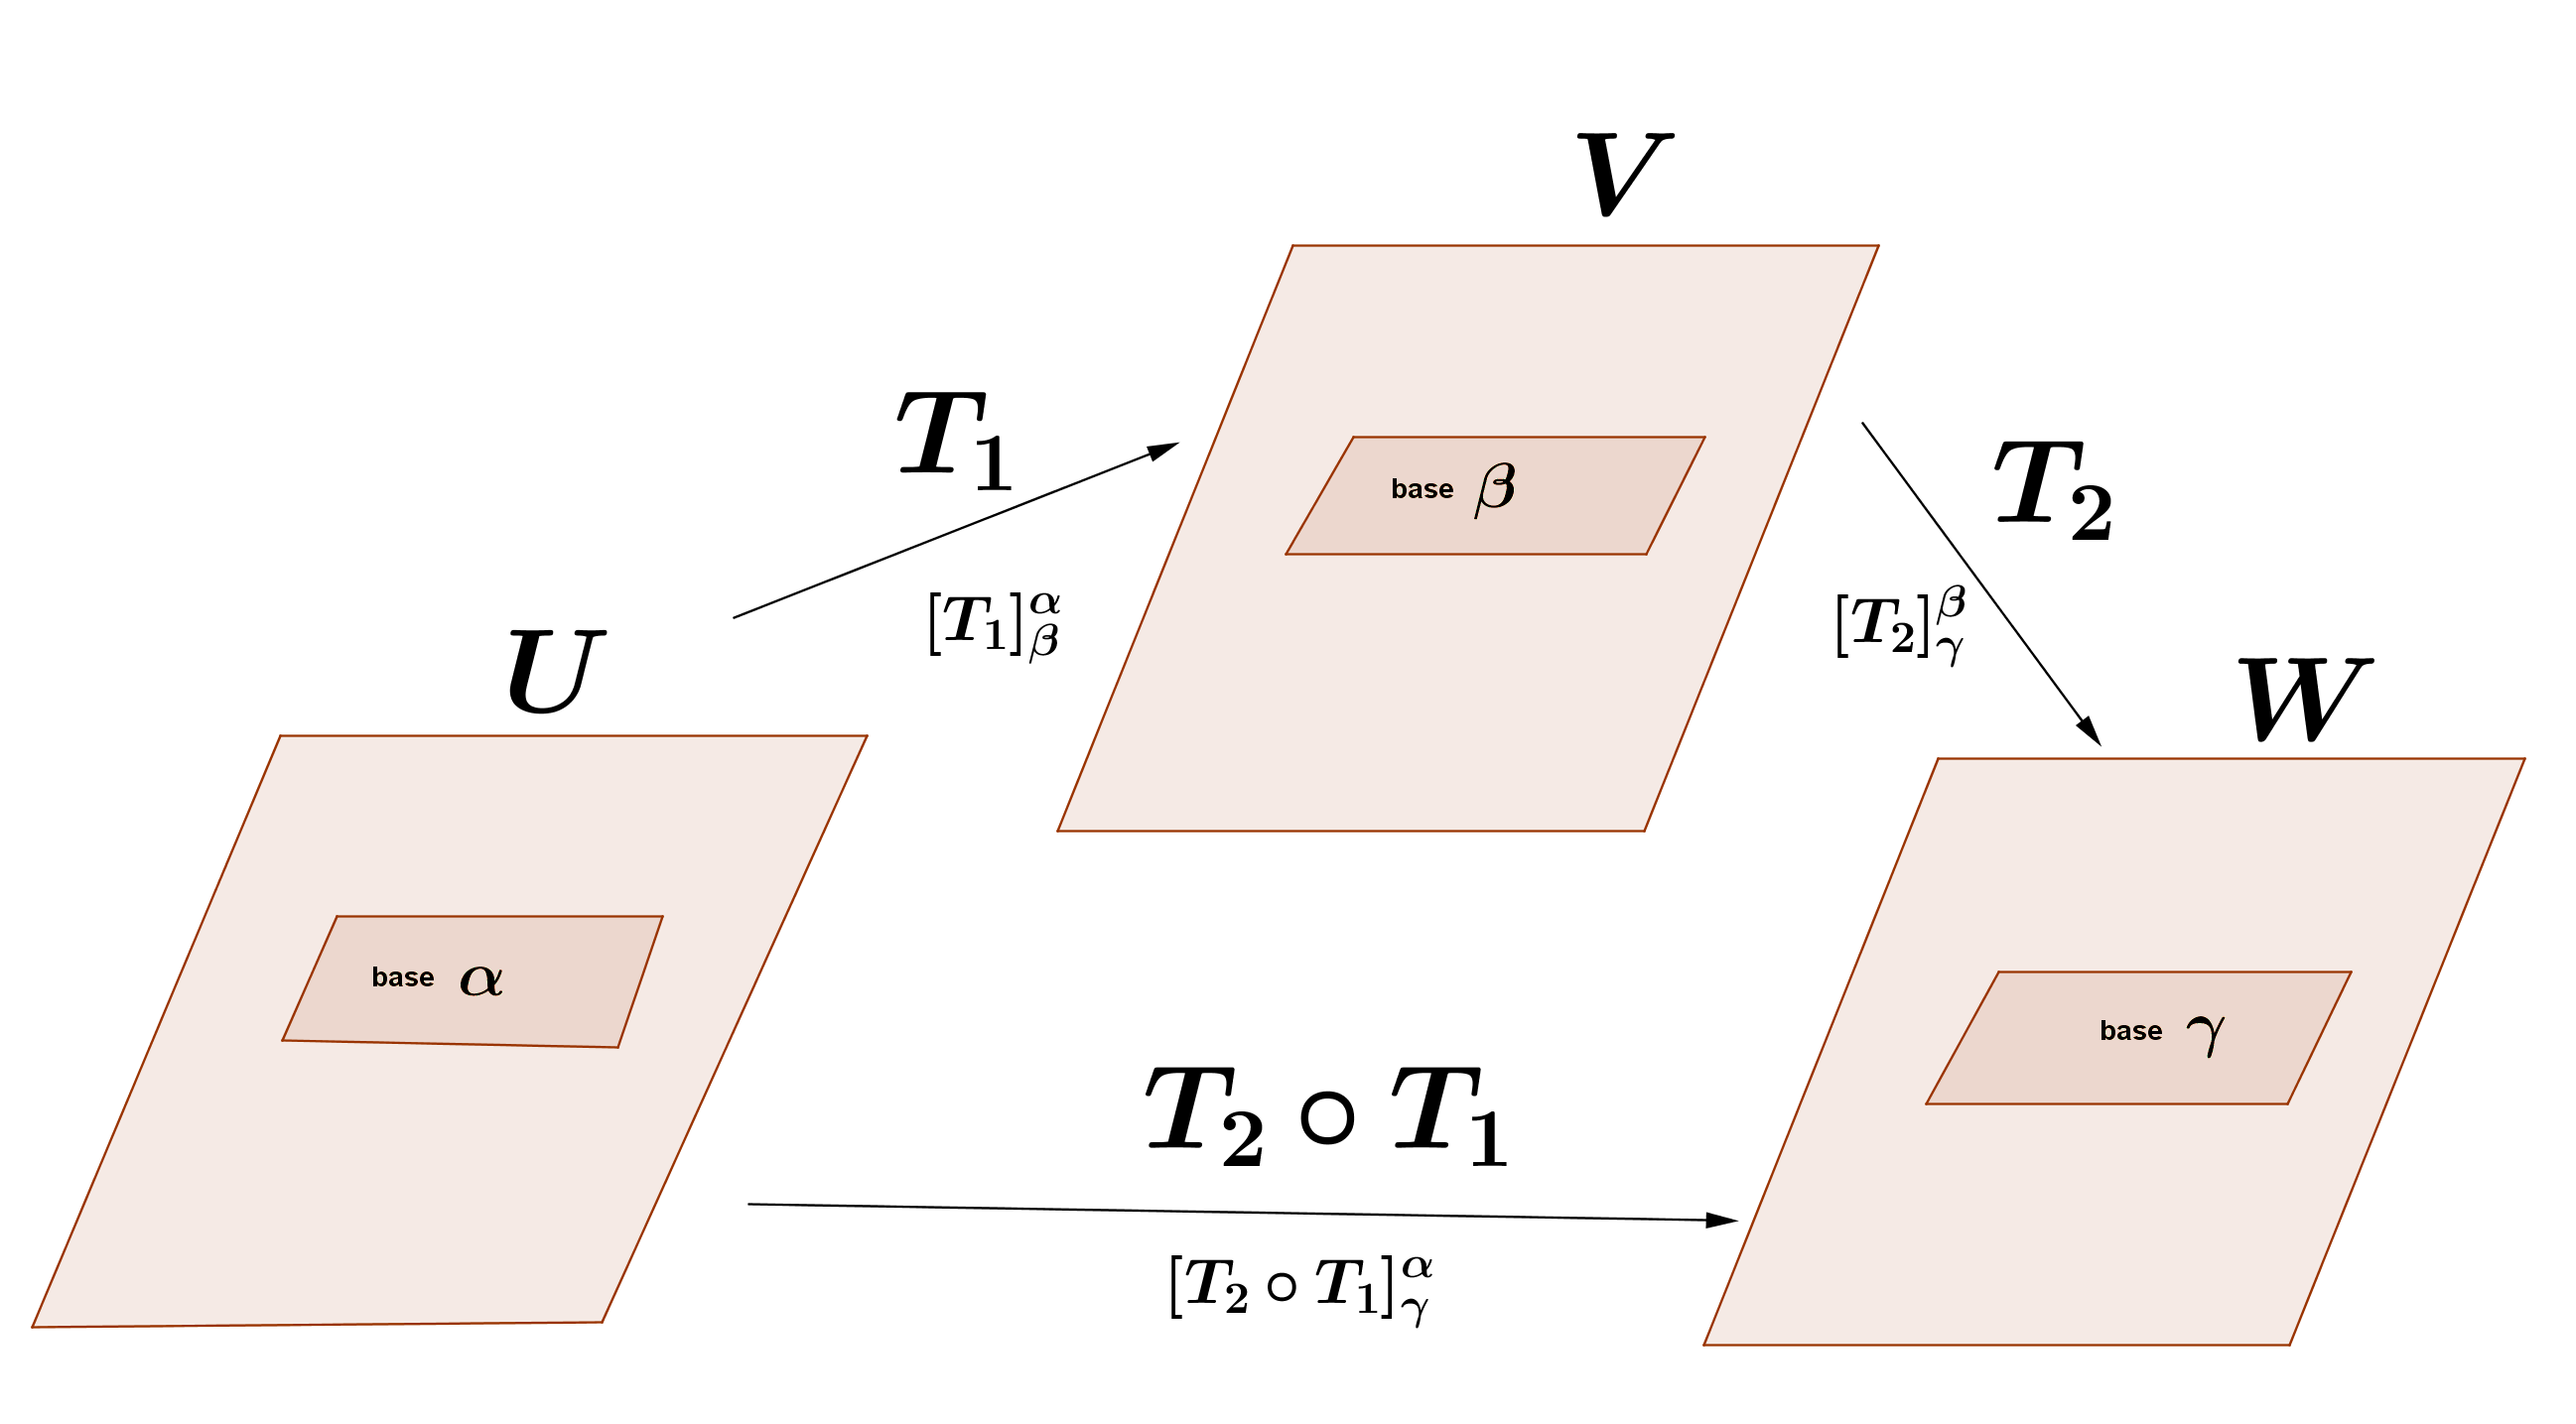
\includegraphics[width=0.8\textwidth]{chapters/matriz_trans_linear/img/composicao}
\caption{\footnotesize{Matriz da composição de duas transformações lineares}}
\label{fig:exp}
\end{figure}


\noindent\textit{\textbf{Demonstração.}} Queremos mostrar que $[T_2 \circ T_1]_{\gamma}^{\alpha}=[T_2 ]_{\gamma}^{\beta} \cdot[T_1]_{\beta}^{\alpha}$. Para isso note que pelo \textbf{Teorema 1} temos
\begin{equation}
[(T_2 \circ T_1)(u)]_{\gamma}=[T_2 \circ T_1]_{\gamma}^{\alpha}[u]_{\alpha}\;\;  e \;\; [(T_2 ( T_1(u))]_{\gamma}=[T_2 ]_{\gamma}^{\beta}[T_1(u)]_{\beta}. \label{teo21}
\end{equation}

Como $(T_2 \circ T_1)(u)=(T_2 ( T_1(u))$, segue  que
\begin{equation}
[T_2 \circ T_1]_{\gamma}^{\alpha}[u]_{\alpha}=[T_2 ]_{\gamma}^{\beta}[T_1(u)]_{\beta}.\label{teo22}
\end{equation}

Mas, por outro lado, também pelo \textbf{Teorema 1}, vem que

\begin{equation}
[T_1(u)]_{\beta}=[T_1]_{\beta}^{\alpha}[u]_{\alpha}.\label{teo23}
\end{equation}

Substituindo \eqref{teo23} em \eqref{teo22}, obtemos:
\begin{equation}
[T_2 \circ T_1]_{\gamma}^{\alpha}[u]_{\alpha}=[T_2 ]_{\gamma}^{\beta}[T_1]_{\beta}^{\alpha}[u]_{\alpha}.\label{teo24}
\end{equation}

Pela unicidade das coordenadas do vetor $u$ em relação a base $\alpha$, segue que
\begin{equation*}
[T_2 \circ T_1]_{\gamma}^{\alpha}=[T_2 ]_{\gamma}^{\beta}[T_1]_{\beta}^{\alpha},
\end{equation*}
como queríamos demonstrar.

\vspace{0.5cm}
Como consequência do \textbf{Teorema 2} resulta que se $T$  é uma transformação linear inversível, então a matriz da transformação inversa $T^{-1}$  pode ser obtida calculando a matriz inversa  da matriz de $T$. Isso é o que afirma o próximo corolário.

\vspace{0.5cm}
\noindent\textbf{Corolário 1.} Se  $T: U \rightarrow V$  é uma transformação linear inversível, ou seja $T$ é um isomorfismo, e $\alpha$ e   $\beta$ são  bases de $U$ e $V$, então  $T^{-1}: V \rightarrow U$ é uma transformação linear e $$[T^{-1} ]_{\alpha}^{\beta} = \left( [T]_{\beta}^{\alpha}\right)^{-1}.$$



\subsection{Matrizes Semelhantes}

Seja  $T:U \rightarrow U$ uma transformação linear e considere $\alpha$ e $\beta$ bases distintas de  $U$.  Então,  podemos obter uma matriz de $T$ em relação a base $\alpha$,  $[T]_{\alpha}^{\alpha}$; e uma matriz de $T$ em relação a base $\beta$,    e  $[T]_{\beta}^{\beta}$.  Uma pergunta importante a se fazer sobre essas duas matrizes  é a seguinte: qual a relação entre as matrizes $[T]_{\alpha}^{\alpha}$ e $[T]_{\beta}^{\beta}$?

Para responder a essa questão, considere  a \textbf{Figura 3.}

\begin{figure}[h!]
\center
% \includegraphics[width=1.0\textwidth]{chapters/matriz_trans_linear/img/semelhanca1}
\caption{\footnotesize{}}
\label{fig:exp}
\end{figure}

Note que as  transformações identidade $I_1$ e $I_2$ possuem matrizes em relação as bases $\alpha$ e $\beta$, $[I_1]_{\alpha}^{\beta}$  e $ [I_2]_{\beta}^{\alpha}$, respectivamente. Note ainda que podemos escrever  $T$ como a transformação composta $$ T=I_2 \circ T \circ I_1.$$

Dessa forma, obtemos
$$ [T]_{\beta}^{\beta}=[I_2 \circ T \circ I_1]_{\beta}^{\beta}.$$

Segue do \textbf{Teorema 2} que
$$ [T]_{\beta}^{\beta}=[I_2]_{\beta}^{\alpha} [ T ]_{\alpha}^{\alpha} [ I_1]_{\alpha}^{\beta}.$$

Como $[ I_1]_{\alpha}^{\beta}=([I_2]_{\beta}^{\alpha})^{-1}$, pois são matrizes mudança de base entre as bases $\alpha$ e $\beta$ e vice-versa; fazendo $P= [I_2]_{\beta}^{\alpha}$, obtemos

$$[T]_{\beta}^{\beta}=P[ T ]_{\alpha}^{\alpha}P^{-1}.$$

Isto significa que as matrizes $[T]_{\alpha}^{\alpha}$ e $[T]_{\beta}^{\beta}$ são \textit{matrizes semelhantes}.

\vspace{0.3cm}

Dizemos que duas matrizes $A$ e $B$ de mesma ordem $n$  são semelhantes, se existe uma matriz $P$, também de  ordem $n$,   invertível  e tal que $$A=P^ {-1}BP.$$


Matrizes semelhantes são importantes porque compartilham, entre outras propriedades, a de possuirem o mesmo determinante e  os mesmos autovalores. No nosso contexto, isso significa que o determinante da matriz $[T]_{\alpha}^{\alpha}$ é igual ao determinante da matriz $[T]_{\beta}^{\beta}$, que é igual ao determinante da matriz da transformação $T$ em qualquer base de $U$. A relevância desse resultado está no fato de que podemos determinar uma  base  de $U$ na qual a matriz de $T$ possa ser a mais simples possível. Por exemplo, uma matriz diagonal.  O problema de determinar uma base do espaço vetorial $U$ para a qual a transformação linear $T:U \rightarrow U$ seja uma matriz diagonal é um problema central nesse curso e será estudado mais adiante.
